\documentclass{acm_proc_article-sp}

\RequirePackage[T1]{fontenc}
\usepackage{pgf}
\usepackage{tikz}
\usepackage{listings}
\numberofauthors{3}
\author{
\alignauthor
Jedrzej Fulara\\
\affaddr{Institute of Informatics}\\
\affaddr{University of Warsaw}\\
\affaddr{ul. Banacha 2}\\
\affaddr{02-097 Warsaw, Poland}\\
\email{fulara@mimuw.edu.pl}
\alignauthor
Krzysztof Jakubczyk\\
\affaddr{Institute of Informatics}\\
\affaddr{University of Warsaw}\\
\affaddr{ul. Banacha 2}\\
\affaddr{02-097 Warsaw, Poland}\\
\email{jakubczyk@mimuw.edu.pl}
\alignauthor
Aleksy Schubert\\
\affaddr{Institute of Informatics}\\
\affaddr{University of Warsaw}\\
\affaddr{ul. Banacha 2}\\
\affaddr{02-097 Warsaw, Poland}\\
\email{alx@mimuw.edu.pl}
}
\title{On Compiling JML Specifications into Bytecode}
\begin{document}
\maketitle


%\section{What should be in paper}
%\begin{itemize}
%	\item What is JML
%	\item What is BML
%	\item Why is translation needed??
% \item Why the tool needed?? (JVM -> VM) BML can be used to different languages, JML to one??
%	\item The tool isn't built on any existing comipler.
%	\item As input we get source file with JML annotations and compiled class file.
%	\item Therefore we can't used optimised bytecode (problem with loops, assertions etc.)
%	\item Optimized bytecode may be used for more general annotations eg. method invariants.
%	\item Detecting loops in bytecode
%	\item Description of matching source code with bytecode loops
%	\item Non-trivial example
%\end{itemize}

\section{Detecting Loops in Bytecode}\label{loopDetection}
To be able to compile the JML loop invariants, one should detect in the bytecode the corresponding loop. The created BML annotation should be associated with the bytecode instruction that represents the loop condition. Note that the loop condition is translated into multiple bytecode instructions. We are interested in the last one (comparison). A loop can be translated in one of the following ways:

\begin{figure}[h]
\centering{
\begin{tikzpicture}[shorten >=1pt,->]
\tikzstyle{vertex}=[circle,draw=blue!50,fill=blue!20,thick,minimum size=17pt,inner sep=0pt]
\foreach \name/\text/\y in {s/.../1, a/a/2, b/b/3, body/.../4, c/c/5, d/d/6, e/.../7}
\node[vertex] (G-\name) at (0,-\y) {$\text$};
\foreach \from/\to in {s/a,b/body,body/c,c/d,d/e}
\draw (G-\from) -- (G-\to);
\draw (G-a) to[out=315,in=45] (G-c);
\draw (G-d) to[out=135,in=225] (G-b);

\foreach \name/\text/\y in {s/.../1, a/a/2, b/b/3, body/.../4, c/c/5, d/d/6, e/.../7}
\node[vertex] (Q-\name) at (4,-\y) {$\text$};
\foreach \from/\to in {s/a,a/b,b/body, body/c, d/e}
\draw (Q-\from) -- (Q-\to);
\draw (Q-b) to[out=315,in=45] (Q-d);
\draw (Q-c) to[out=135,in=225](Q-a);
\end{tikzpicture}
\caption{Two ways of compiling loops.}
}
\end{figure}
In the first scenario, in the vertex \textit{a}, an unconditional jump (goto) to the vertex \textit{c} is done (vertex \textit{c} denotes loading the condition). In \textit{d} the condition is checked, and if it is fulfilled, we jump back to \textit{b}. Between \textit{b} and \textit{c} is the loop body. The annotation should be added to the vertex \textit{d}. In the second approach, the condition is tested at the beginning (\textit{a} puts the condition on the stack and \textit{b} checks it. If it is fulfilled, we enter the loop, otherwise we jump out). In \textit{c} an unconditional jump back to \textit{a} is done. The BML annotation should be associated with the instruction in the vertex \textit{a}.

\texttt{Do-while} loops and loops with always true condition (i.e. \texttt{while(true)\{...\}} or \texttt{for(;;)\{...\}} are usually compiled in another way:

\begin{figure}[h]
\centering{
\begin{tikzpicture}[shorten >=1pt,->]
\tikzstyle{vertex}=[circle,draw=blue!50,fill=blue!20,thick,minimum size=17pt,inner sep=0pt]
\foreach \name/\text/\x in {s/.../1, a/a/2, body1/.../3, b/b/4, body2/.../5, c/c/6, d/.../7}
\node[vertex] (G-\name) at (\x,0) {$\text$};
\foreach \from/\to in {s/a,a/body1, body1/b, b/body2, body2/c}
\draw (G-\from) -- (G-\to);
\draw (G-b) to[out=315,in=225] (G-d);
\draw (G-c) to[out=135,in=45] (G-a);
\end{tikzpicture}
\caption{Compiling \texttt{do-while} loop.}}
\end{figure}
Before entering the loop (between \textit{a} and \textit{c}), no condition is checked. There might be some \texttt{break} inside (vertex \textit{b}).
In this cases, the annotation should be added to \textit{a} (start of the loop). The Jml2Bml compiler covers all the cases described above. It tries to detect the first kind of loop. If it fails, tries to detect the second one. At the end checks the \texttt{do - while} case. In the first case:
\begin{itemize}
\item{assume that the tested instruction is in vertex \textit{c}. Consider all incoming edges that start in a vertex \textit{v}, which is before \textit{c}}
\item{if there are no such vertices, return null (tested instruction is not the \textit{c} vertex in the first kind loop)}
\item{else take this \textit{v} that has the longest jump to \textit{c} (other jumps come from some continue instructions inside the loop). This is \textit{a} from our graph,}
\item{look at the next instruction. This is our \textit{b}. Find the longest backward jump. It is our vertex \textit{d}}
\item{return d}
\end{itemize}
If no loop of the first kind was detected for an instruction, try to detect the second kind:
\begin{itemize}
\item{assume that the tested instruction is \textit{a}.}
\item{if the instruction has less than two incomming edges - return null}
\item{find \textit{v} that is after \textit{a} and has the longest jump to it. This is \textit{c} from our graph.}
\item{look at the next instruction \textit{d}.}
\item{find such \textit{u} that there exist an edge (\textit{u},\textit{d}) and \textit{u} is between \textit{a} and \textit{d} and there is no such \textit{u'} that \textit{u'} is between \textit{a} and \textit{u} and there is an edge (\textit{u'},\textit{d}). This is candidate for \textit{b}}
\item{if at \textit{u} is an unconditional jump (goto), then this is a break - this is the case of loop with always true condition. Return \textit{a}}
\item{else (at \textit{u} is a conditional jump) - \textit{u} is really our \textit{b}. Return it.}
\end{itemize}
If both cases described above fail, the algorithm tries to detect the \texttt{do - while} loop. We simply check if
\begin{itemize}
\item{there is a backward jump from the tested instruction to some \textit{a}}
\item{if yes, assuming that cases 1 and 2 failed, return \textit{a} as the beginning of the loop}
\end{itemize}

\section{Matching Bytecode Loops with Source Loops}
Let us take any source method that has loop with JML invariant and bytecode corresponding to this method. The compiler used to generate the bytecode may have used some optimizations. Unfortunately this causes some problems. Here are some exemplary loop optimizations:
\begin{itemize}
	\item loop unwinding (loop unrolling)\\
In this case invariant should be put in every copy of the loop. But the invariant may need a change.
	\item loop interchange\\
If internal loop invariant depended on external loop variables - this invariant must also be translated.
	\item code-motion\\
Some part of code may be moved before the loop. What if invariant depended on it?
\end{itemize}
When we want to add BML specifications to optimized bytecode, we have to know the optimizations that were used. There are two solutions of this problem:
\begin{itemize}
	\item Include the JML to BML compiler in existing Java compiler application.
	\item Use non-optimizing compiler.
\end{itemize}

\section{Conclusion/Introduction??}
Java Virtual Machine can be used with languages different than Java. Few examples:
\begin{itemize}
	\item Jython - the Python Java implementation
	\item JRuby - the Ruby Java implementation
	\item Jacl - the Tcl Java implementation
	\item Rhino - the JavaScript Java implementation
\end{itemize}
At SugarCon 2008, Sun Microsystems CEO Jonathan Schwartz said that "we are just going to take the 'J' off the 'JVM' and just make it a 'VM'.". Therefore there will be a global trend with support of companies to use JVM with other languages. Java language has JML with proper tools that can be used to verify programs - check their correctness or find errors. Most of them operates on source code. Bytecode itself has a verification algorithm but the verification is done only to ensure that the loaded bytecode will not cause the crash of the JVM. Verification algorithm includes:
\begin{itemize}
	\item checking that all arguments on the operand stack are legal
	\item ensuring that all types of variables passed to methods are correct
	\item checking that all load and store operations have correct types
\end{itemize}
Unfortunately programming errors are not checked. The BML language with proper verification tools can take over all qualities of source code verification using JML. The main advantage of such approach is that the verification itself will not be limited only to Java language - but can be used with any language that is compilled to JVM bytecode. There are mainly three sets of tools needed:
\begin{itemize}
	\item bytecode verification tools that use BML annotations
	\item modelling languages (such as JML for Java) for other programming languages
	\item compilers that compile programs to JVM bytecode along with annotation compilers
\end{itemize}
Our Jml2Bml is designed to be a part of this scheme.

\section{Architecture Description}
In this section we present the overview of the architecture of Jml2Bml compiler. The \textit{Jml2Bml} compiler uses \textit{OpenJml} to parse the Java source code together with the JML annotations. To insert generated BML annotations, the \textit{BMLLib} library is used. The dependencies between internal packages and \textit{Jml2Bml} and \textit{BMLlib} are presented in figure \ref{packages}.

The \texttt{jml2bml.main} package provides the entry point to the application. JML annotations from given source file will be translated and inserted into corresponding \texttt{class} file. Functions to access some bytecode information are located in \texttt{jml2bml.bytecode} and helpers to \textit{BMLlib} are collected in \texttt{jml2bml.bmllib}. The \texttt{jml2bml.rules} package contains translation rules for different aspects of JML. It should be easy to add new rules in the future. Classes for traversing the Java abstract syntax tree can be found in \texttt{jml2bml.ast}. In \texttt{jml2bml.symbols} implementation of symbol table can be found. The \texttt{jml2bml.engine} package contains the core translating mechanism. The whole tree is traversed and in each node all defined translation rules are applied. It allows also to register new rules in a very simply way, what is an important issue in case of implementing new features in the future.
\begin{figure}[h]
\centering{
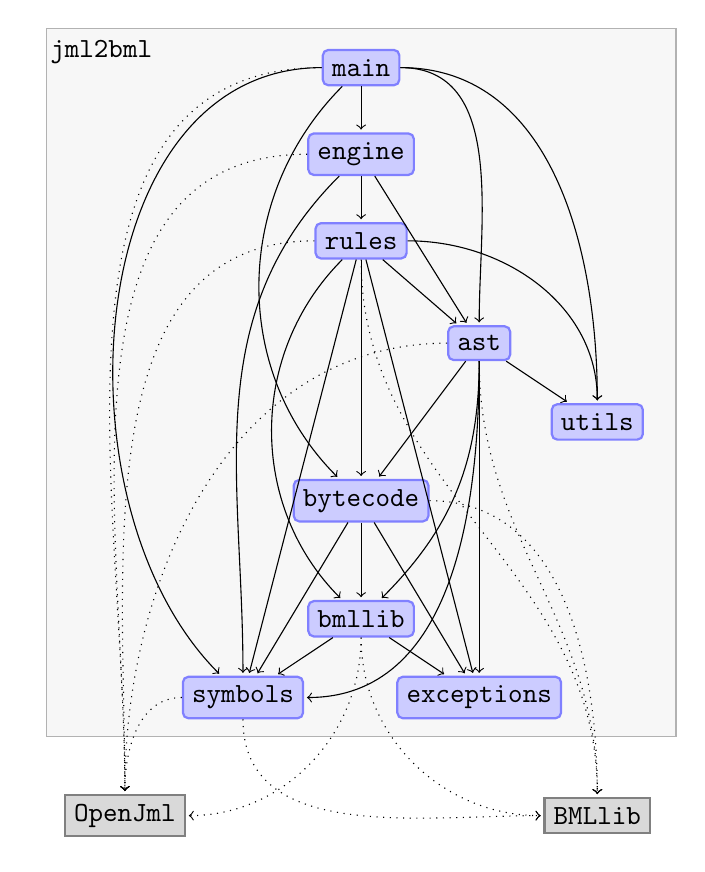
\begin{tikzpicture}[shorten >=1pt,->]
\
\tikzstyle{vertex}=[rectangle,draw=blue!50,fill=blue!20,thick,rounded corners = 2pt]
\filldraw[draw=black!30,fill=black!3] (-1,7.5) rectangle (7,-1.5);
%\draw (-0.9,7.2) node[right]{\textbf{\texttt{jml2bml}}};
\node (label) at (-0.3,7.2){\textbf{\texttt{jml2bml}}};
\node[vertex] (main) at (3,7) {\texttt{main}};
\node[vertex] (engine) at (3,5.9) {\texttt{engine}}  ;
\node[vertex] (rules) at (3,4.8) {\texttt{rules}}  ;
\node[vertex] (ast) at (4.5,3.5) {\texttt{ast}}  ;
\node[vertex] (utils) at (6,2.5) {\texttt{utils}};
\node[vertex] (bytecode) at (3,1.5) {\texttt{bytecode}};
\node[vertex] (bmllib) at (3, 0) {\texttt{bmllib}};
\node[vertex] (exceptions) at (4.5, -1) {\texttt{exceptions}};
\node[vertex] (symbols) at (1.5, -1) {\texttt{symbols}};
\draw (main) -- (engine);
\draw (engine) -- (rules);
\draw (rules) --(ast);
\draw (engine) -- (ast) ;
\draw(ast) -- (utils) ;
\draw(ast) -- (bytecode);
\draw (ast) to[out=270,in=45] (bmllib);
\draw (ast) -- (exceptions);
\draw (main) to[out=0,in=90] (ast);
\draw (rules) to[out=0,in=90] (utils);
\draw (rules) -- (symbols);
\draw (rules) -- (exceptions);
\draw (rules) to[out=225,in=135] (bmllib);
\draw (main) to[out=0,in=90] (utils);
\draw (main) to[out=225,in=135] (bytecode);
\draw (main) to[out=180,in=135] (symbols);
\draw (engine) to[out=225,in=90] (symbols);
\draw (ast) to[out=270,in=0] (symbols) ;
\draw (rules) -- (bytecode);
\draw (bytecode) -- (bmllib) ;
\draw (bytecode) -- (exceptions) ;
\draw (bytecode) -- (symbols) ;
\draw (bmllib) -- (exceptions) ;
\draw (bmllib) -- (symbols) ;
\tikzstyle{external}=[rectangle,draw=black!50,fill=black!15,thick]
\node[external] (BmlLib1) at  (6, -2.5) {\textbf{\texttt{BMLlib}}};
\node[external] (openJml) at  (0, -2.5) {\textbf{\texttt{OpenJml}}};
\draw[dotted] (main) to[out=180,in=90] (openJml);
\draw[dotted] (engine) to[out=180,in=90] (openJml);
\draw[dotted] (rules) to[out=180,in=90] (openJml);
\draw[dotted] (rules) to[out=270,in=90] (BmlLib1);
\draw[dotted] (ast) to[out=270,in=90] (BmlLib1);
\draw[dotted] (ast) to[out=180,in=90] (openJml);
\draw[dotted] (bytecode) to[out=0,in=90] (BmlLib1);
\draw[dotted] (bmllib) to[out=270,in=0] (openJml);
\draw[dotted] (bmllib)  to[out=270,in=180] (BmlLib1);
\draw[dotted] (symbols) to[out=180,in=90] (openJml);
\draw[dotted] (symbols) to[out=270,in=180] (BmlLib1);
\end{tikzpicture}
\caption{The dependency graph of the \textit{Jml2Bml} packages. Dotted lines denote access to external libraries.}}
\label{packages}
\end{figure}
\section{Translation Principles}
Tutaj bedziemy opisywac,ze nie uzywamy tablicy linii, bierzemy kod bez optymalizacji itp.
\section{An Example of Using The\\Compiler}
This section provides an example demonstrating the result of launching the \textit{Jml2Bml}.
\subsection{Source Code}
Consider the class presented in figure \ref{source}. This is an excerpt of a class which implements a sequence of objects. We present here only one method that replaces in the \texttt{list} array all occurences of its first parameter with the second one.

The presented code, apart from standard Java statements, contains also specifications in the JML. There is a precondition (\texttt{requires ...}) for the method \texttt{replace} defined. It requests that every time the method is invoked, the field \texttt{list} it not \texttt{null}. The next three lines (starting with \texttt{ensures} constitute the method postcondition. It states that, if the precondition was fullfiled, then the method result is true if and only if there was an element in the \texttt{list} which value has been updated from \texttt{o1} to \texttt{o2}. Note that the postcondition makes use of some JML features, like \texttt{$\backslash$result}, \texttt{$\backslash$old} or \texttt{$\backslash$exists}. This postcondition does not describe all properties of this method. For example an implementation that replaces all elements in the \texttt{list} up to the first occurence of \texttt{o1} with \texttt{o2} will fulfill this specification.

In additition to specification describing input - output behaviour of the method, also the loop implementing the \texttt{replace} method is annotated. The \texttt{loop\_invariant} clause contains the invariant: a formula that should hold at the beginning of the loop body at each loop iteration. In this example it states that in iteration \texttt{i} there are no occurences of \texttt{o1} in \texttt{list} on positions before \texttt{i}. The annotation \texttt{decreases} describes the loop variant. It specifies an expression (in this case \texttt{list.length - i}) which value is decreased in each loop iteration by at least one.


\lstset{language=java, morekeywords={requires,ensures,\result,\exists,\old,loop_invariant,\forall,==>, decreases},
        basicstyle=\small,commentstyle=\small,moredelim=*[s][\small]{/*@}{*/}}
\begin{figure}
\centering{
\begin{lstlisting}
public class List {

  private Object[] list;

  /*@ requires list != null;
    @ ensures \result ==(\exists int i;
    @ 0 <= i && i < list.length &&
    @ \old(list[i]) == o1 && list[i] == o2);
    @*/
  public boolean replace(Object o1, Object o2){
    /*@
      @ loop_invariant i <= list.length
      @ && i >=0 && (\forall int k;0 <= k
      @ && k < i ==> list[k] != o1);
      @ decreases list.length - i;
      @*/
    for (int i = 0; i < list.length; i++) {
      if (list[i] == o1) {
        list[i] = o2;
        return true;
      }
    }
    return false;
  }
}
\end{lstlisting}
}
\caption{An example class \texttt{List.java} containing single method \texttt{replace}.}
\label{source}
\end{figure}
\subsection{Bytecode}
In this section we describe the result of translating the source code from Figure \ref{source}. Since the binary class files are not human readable, we rely on its textual representation obtained from the BMLlib. The Figure \ref{bytecode} shows the translated \texttt{replace} method together with BML annotations inserted by our Jml2Bml compiler. Lines 0 and 1 correspond to initialization the \texttt{i = 0}. The loop is located between lines 2 and 33. Lines 5 - 12 represent the \texttt{if} statement, 15 - 23 correspond to lines ??? from the source code. Loading loop condition parameters is located in lines 27 - 32 and 33 performs the loop condition comparison. 

The \texttt{requires-enusers} pair is translated into input-output behaviour BML specifications located just before the method code. Loops specifications are located after line 32 in the presented listing. The Jml2Bml compiler detects loops in the bytecode and inserts the annotation before the statement representing the loop condition. In this case it is the \texttt{if\_icmplt} instruction comparing \texttt{i} and \texttt{list.length}. For more details about detecting loops refer to section \ref{loopDetection}. The modifies clause describes set of variables modified by the loop. Currently, because of \textit{OpenJML} limitations it is not supported by our compiler (the default value \texttt{everything} will be inserted).
\begin{figure}
\lstset{basicstyle=\small}

\begin{lstlisting}
/*
 * \requires true
 *  {|
 *   \precondition list != null
 *   \ensures \result ==
 *     (exists int i; 0 <= i && i < list.length
 *       && old_list[i] == o1 && list[i] == o2)
 *  |}
 */
public boolean replace(Object o1, Object o2)
0:    iconst_0
1:    istore_3
2:    goto	   #27
5:    aload_0
6:    getfield	   main.List.list
9:    iload_3
10:   aaload
11:   aload_1
12:   if_acmpne	   #24
15:   aload_0
16:   getfield	   main.List.list
19:   iload_3
20:   aload_2
21:   aastore
22:   iconst_1
23:   ireturn
24:   iinc	   %3	1
27:   iload_3
28:   aload_0
29:   getfield	   main.List.list
32:   arraylength
/*
 * \loop specification
 *   \modifies everything
 *   \invariant i <= list.length &&
 *      i >= 0 &&
 *      (forall int k; 0 <= k &&
 *          k < i==>list[k] != o1)
 *   \decreases list.length - i
 */
33:   if_icmplt	   #5
36:   iconst_0
37:   ireturn

\end{lstlisting}
\label{bytecode}
\caption{The method \texttt{replace} in the \texttt{List.class}}
\end{figure}
\end{document}
